\documentclass[11pt]{beamer}
\usepackage[spanish]{babel}

\usetheme{Berlin}
\usecolortheme{seahorse}

%%%%%%%%%%%%%%%%%%%%%%%%%%%%%%%%%%
%%%%%%%%%%%%%%%%%%%%%%%%%%%%%   %%
%%        Datos Trabajo     %%  %%
%%%%%%%%%%%%%%%%%%%%%%%%%%%%%%%%%%
\newcommand{\titulo}[0]{ASIGNACIÓN A CARGO DEL DOCENTE}
\newcommand{\materia}[0]{Estadística Básica}
\newcommand{\grupo}[0]{BI-BEBA-2002-B2-013}
\newcommand{\unidad}[0]{ACD}


%%%%%%%%%%%%%%%%%%%%%%%%%%%%%%%%%%
%%%%%%%%%%%%%%%%%%%%%%%%%%%%%%%%%%
\usepackage{amssymb}
\usepackage{enumerate}
\usepackage{geometry}
\usepackage{mathtools}
\usepackage{multicol}
\usepackage{soul}

\usepackage{graphicx}
	\graphicspath{ {assets/} }

\usepackage{hyperref}
	\hypersetup{
			pdftex,
		        pdfauthor={bench},
		        pdftitle={\titulo},
		        pdfsubject={\materia},
		        pdfkeywords={\grupo, \unidad, UnADM},
		        pdfproducer={Latex with hyperref, Ubuntu},
		        pdfcreator={pdflatex, or other tool},
			colorlinks=true,
				linkcolor=[rgb]{0,0,0.45},
				urlcolor=cyan,
				filecolor=green,
				citecolor=blue}

%%%%%%%%%%%%%%%%%%%%%%%%%%%%%%%%%%
%%%%%%%%%%%%%%%%%%%%%%%%%%%%%%%%%%

\title[Actividad 1]{
	%
\includegraphics[width=3cm]{../../../assets/logo-unadm} \\
	\bf{\titulo}}

\author{ Benjamín Rivera }
\institute{Universidad Abierta y a Distancia de México \\
	\tiny
	TSU en Biotecnolog\'ia }
\date{\textit{Fecha de entrega:} \today}


%%%%%%%%%%%%%%%%%%%%%%%%%%%%%
%%        Documento         %%
%%%%%%%%%%%%%%%%%%%%%%%%%%%%%%%
\begin{document}
	\begin{frame}
		\maketitle\tiny
		\textit{Materia:} \materia \\
		\textit{Grupo:} \grupo \\
		\textit{Unidad:} \unidad \\
		\textit{Matricula:} ES202105994
		
	\end{frame}

	\begin{frame}{Tabla de contenidos}
		\tableofcontents
	\end{frame}

%%%%%%%%%%%%%%%%%%%%%%%%%%%%%%
%%%%%%%%%%%%%%%%%%%%%%%%%%%%%
%%%%%%%%%%%%%%%%%%%%%%%%%%%%%%
\section{Caso de estudio}
	
	\begin{frame}{Caso de estudio}		
		\par En este proyecto se centrara en explorar cierta característica de los grupos de corales en el mundo, la profundidad a la que estos habitan y se desarrollan.
		
		\begin{figure}[h]
			\centering
				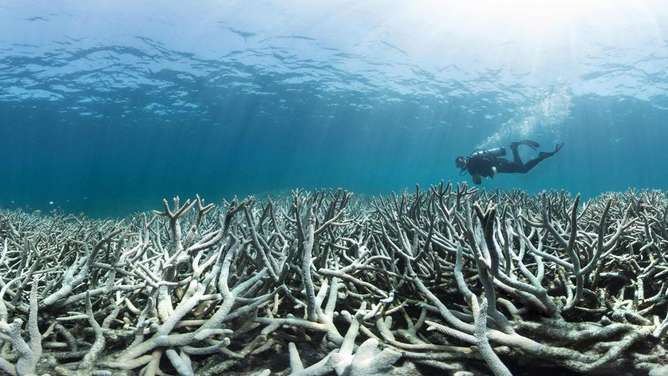
\includegraphics[width=0.5\textwidth]{coral-muerto.jpg}
			\caption{Corales muertos en el Océano Índico \cite{corales muertos}}
			\label{fig: corales muertos}
		\end{figure}
	\end{frame}
	
	\subsection{Relación con la Biotecnología}
	\begin{frame}{Relación con la Biotecnología}
		\par Estoy interesado en estudiar las \textbf{técnicas de repoblación de ecosistemas} usando agentes biológicos. Esto es importante para poder analizar ecosistemas afectados y aquellos que sean sanos, y que posean características similares.
	\end{frame}

%%%%%%%%%%%%%%%%%%%%%%%%%%%%%%
%%%%%%%%%%%%%%%%%%%%%%%%%%%%%
%%%%%%%%%%%%%%%%%%%%%%%%%%%%%%
\section{Datos y análisis}

	\subsection{Base de Datos}
	\begin{frame}{Base de Datos}
		Para este proyecto se usarea la base de datos \cite{db}. De esta podemos obtener la visualización preliminar de la figura~\ref{fig: tabla}.
	
		\begin{figure}[h]
			\centering
				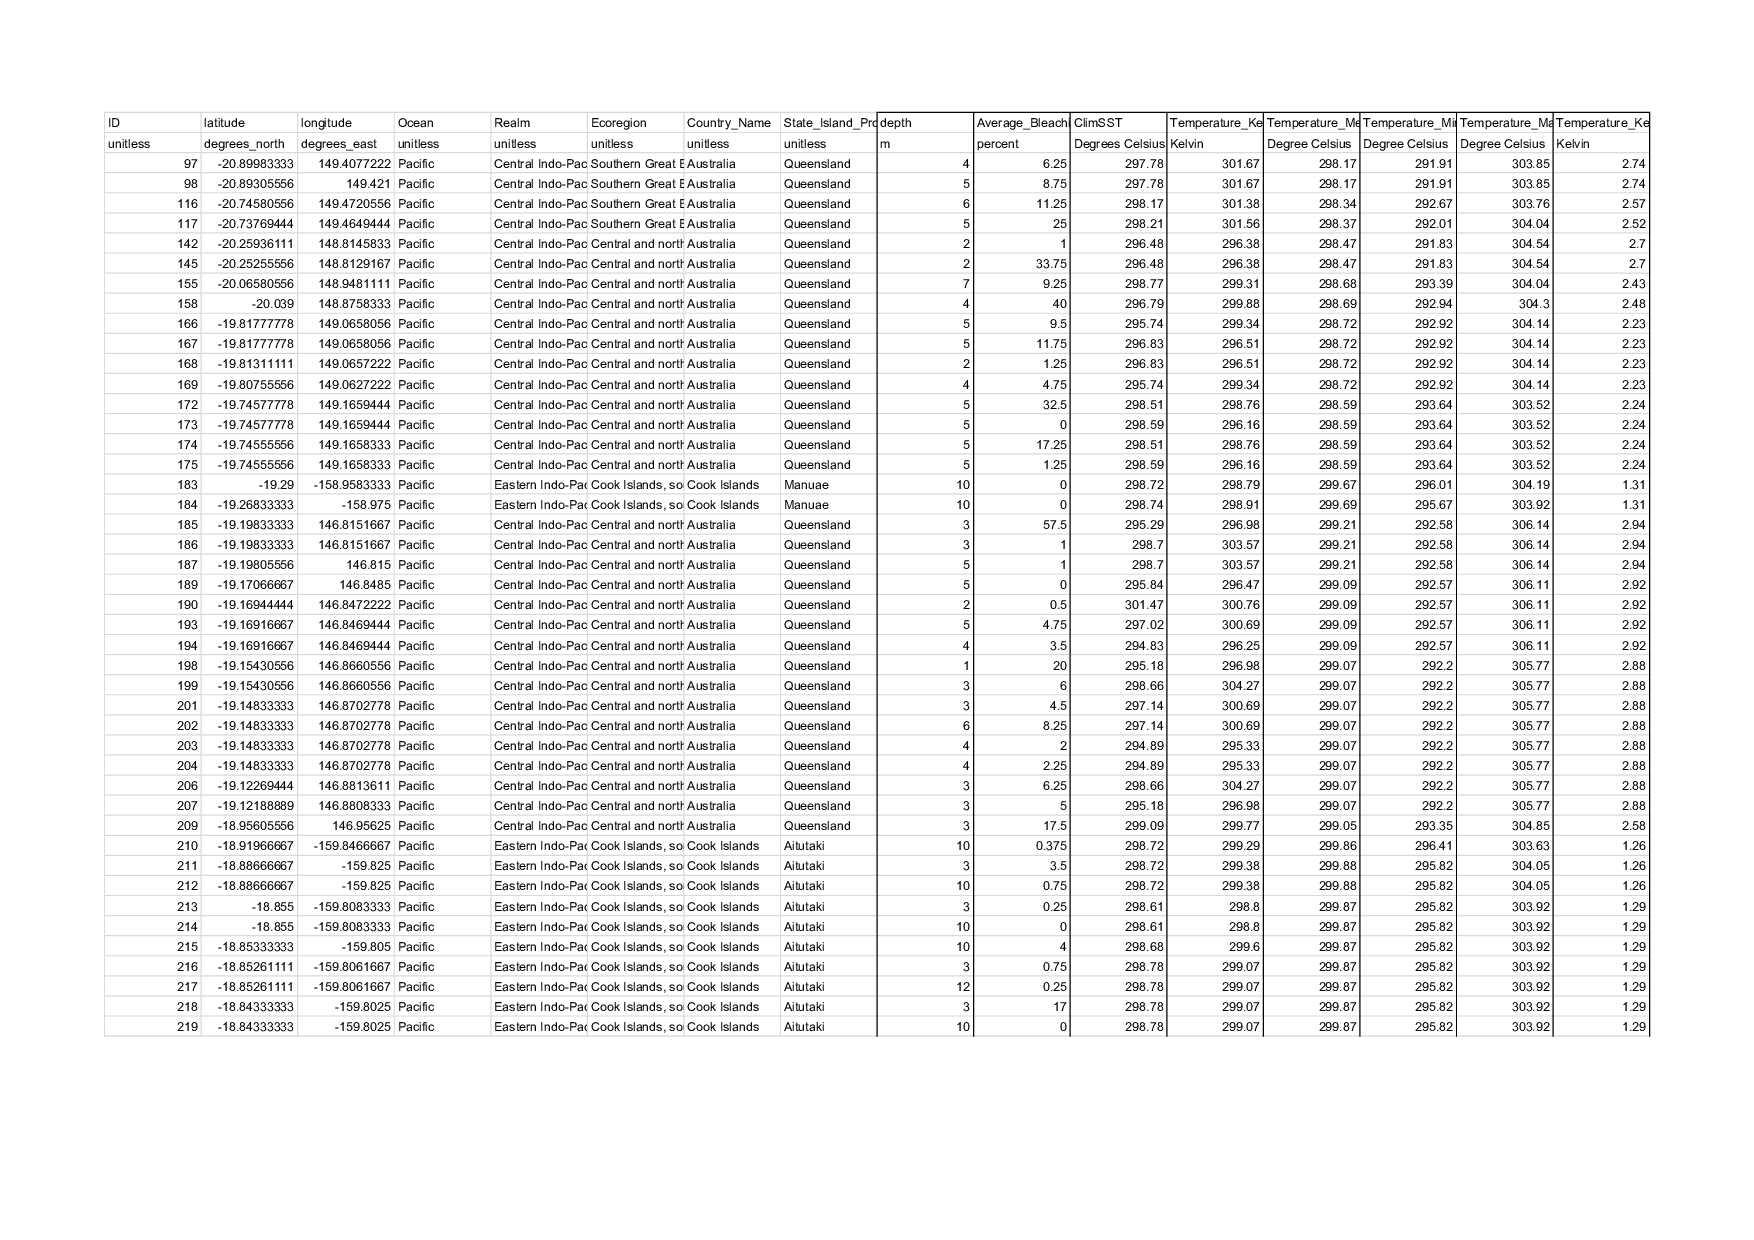
\includegraphics[height=0.5\textheight]{dataset_coral.png}
			\caption{Representación de la información guardada en la base de datos.}
			\label{fig: tabla}
		\end{figure}
	\end{frame}
	\begin{frame}
		\par Esta es una base de datos de la \href{www.bco-dmo.org}{BCO-DM} que recolecta $9,967$ entradas que contienen $46$ características de asentamientos de coral en todo el mundo.
		\par \
		\par Entre estas características se encuentra la \textit{profundidad} (\textbf{depth}), que es la que empezaremos a estudiar en este proyecto.
	\end{frame}
	
	
	\subsection{Frecuencias y gráficas}
	\begin{frame}{Tabla de frecuencias}
		\par Con los entradas de la columna \textit{profundidad} de la base de datos se obtuvieron las siguientes frecuencias y sus gráficas correspondientes.
	
		\begin{figure}[h]
			\centering
				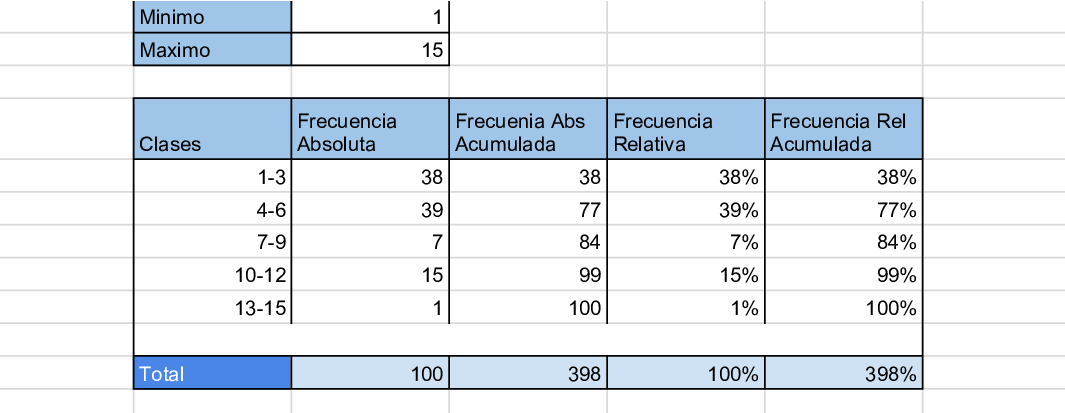
\includegraphics[width=0.6\textwidth]{dataset_coral-frecuencias.png}
			\caption{Tabla de frecuencias de los primeros 100 datos de profundidad de los corales.}
			\label{fig: tabla frecuencia}
		\end{figure}
	\end{frame}
	
	\begin{frame}{Gráficos}
		\begin{figure}[h]
			\centering
				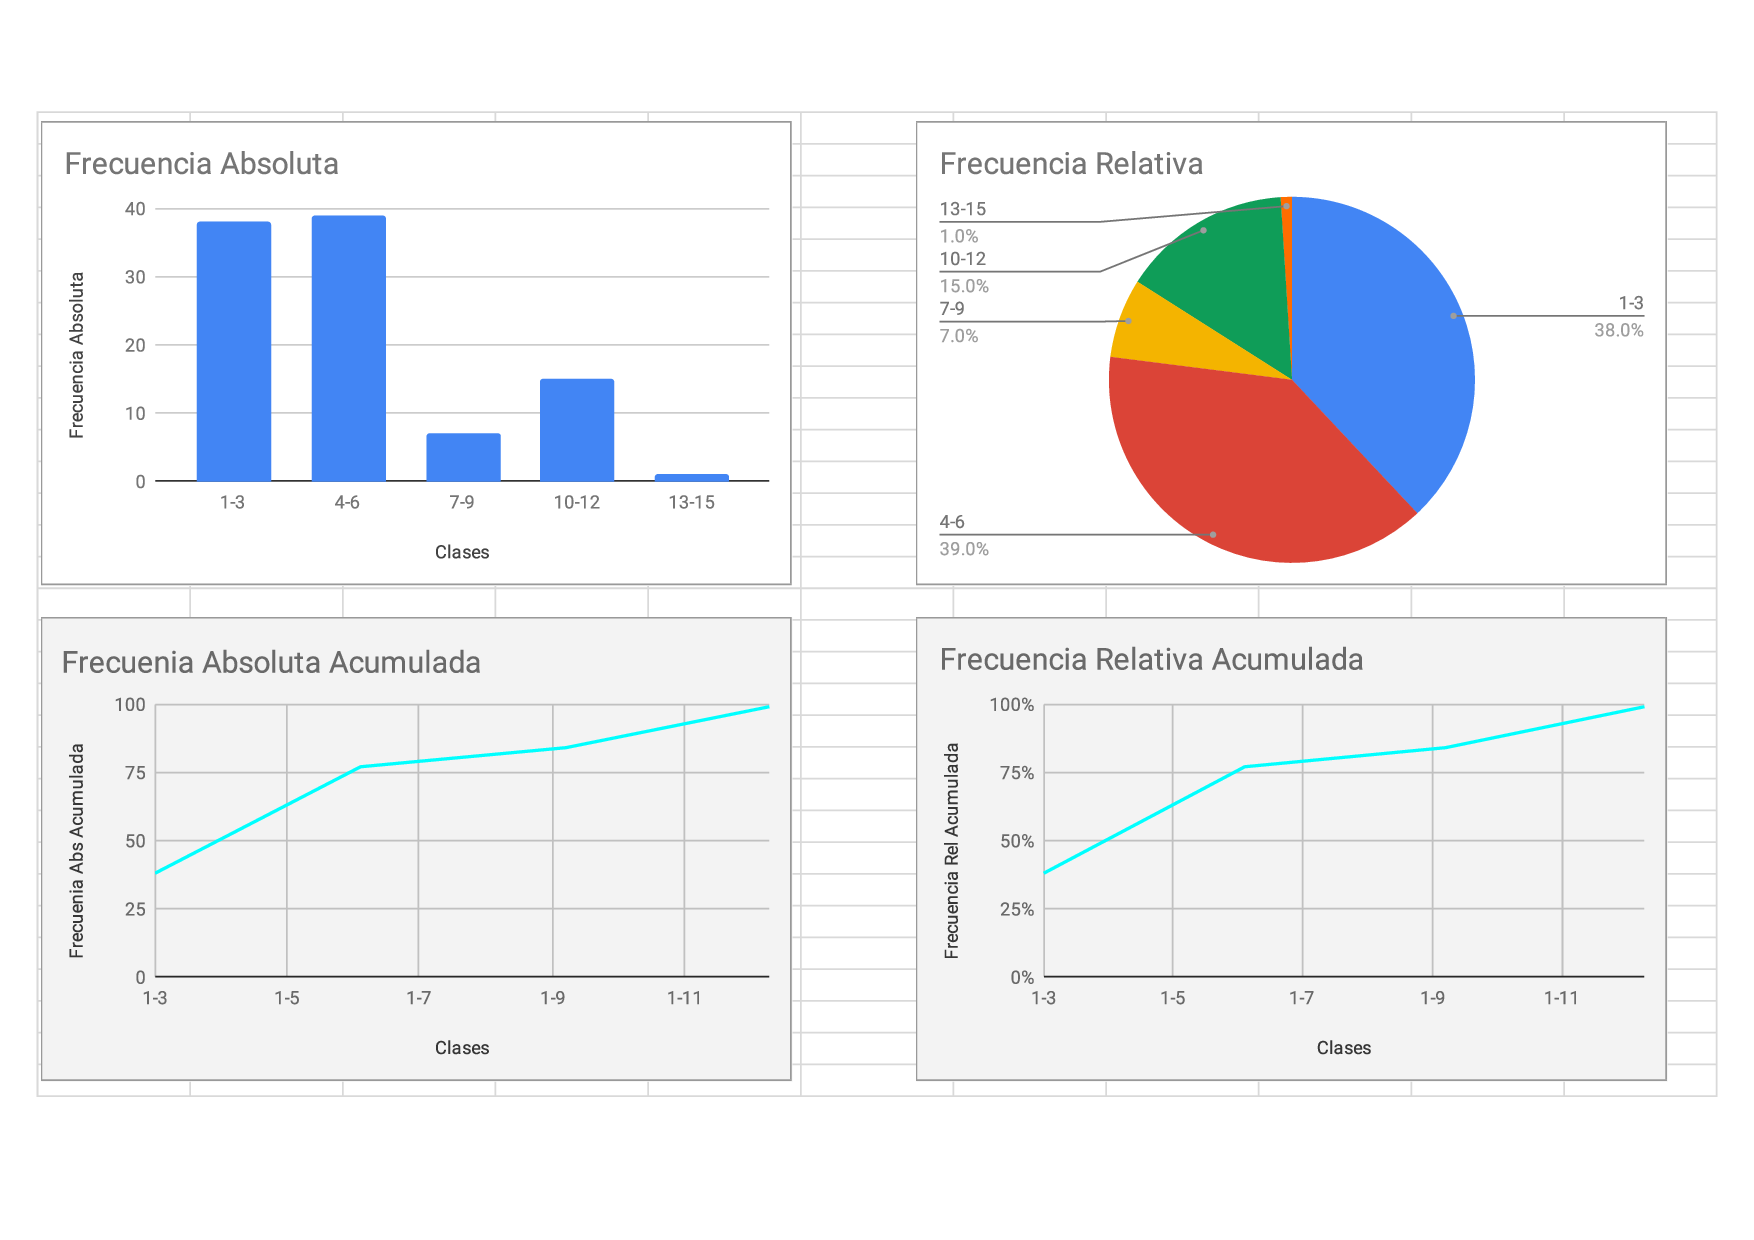
\includegraphics[width=0.7\textwidth]{dataset_coral-graficos.png}
			\caption{Gr\'aficos generados de la tabla de distribuci\'on de frecuencias.}
			\label{fig: graficos}
		\end{figure}
	\end{frame}
	
	
	\subsection{Muestreo, tendencias y dispersión.}
	\begin{frame}{Muestreo de datos}
		Para los demás cálculos de este proyecto debemos seleccionar una muestra. Para esto tomamos un \textit{margen de error} del $10\%$, un \textit{nivel de confianza} de $99\%$ y una población de $9,967$. Con estos datos, y la fórmula vista en clase, obtenemos que la muestra debe ser de $167$ entradas.
		\par Posteriormente la muestra fue seleccionada de manera aleatoria con el uso de sistemas informáticos.
	\end{frame}
	
	\begin{frame}{Medidas de tendencia central}
		Con esta muestra se obtuvieron las siguientes medidas de tendencia central.
		\begin{description}
			\item [Promedio] $6.41$
			\item [Mediana] $6$
			\item [Moda] $5$
		\end{description}
	\end{frame}
	
	\begin{frame}{Medidas de dispersión}
		Y también las siguientes medidas de dispersión.
		\begin{description}
			\item [Desviación Estandar] $3.43$
			\item [Varianza] $11.77$
		\end{description}
	\end{frame}
	


%%%%%%%%%%%%%%%%%%%%%%%%%%%%%%
%%%%%%%%%%%%%%%%%%%%%%%%%%%%%
%%%%%%%%%%%%%%%%%%%%%%%%%%%%%%	
\section{Reporte estadístico}
	\begin{frame}{Reporte estadístico}
		\par Antes de las conclusiones agradezco al encargado de la base de datos que la tiene bastante limpia, lo cual sabemos que no es sencillo de hacer.
		\par \
		\par Respecto al proyecto, podemos ver que la desviación estándar es (relativamente) baja; eso puede implicar que puede haber una zona \textit{segura} donde se desarrollan mejor, para asegurar esto deberíamos de observar la forma de la distribución y verificar la interacción de otras variables.
	\end{frame}



%%%%%%%%%%%%%%%%%%%%%%%%%%%%%%%%
%%         Bibliografia        %%
%%%%%%%%%%%%%%%%%%%%%%%%%%%%%%%%%%
\newpage
\scriptsize
\section{Referencias}
\begin{frame}{Referencias}
	\begin{thebibliography}{X}\tiny
	
		\bibitem{basico1} (s. a.) (s. f.). \textit{Estadística básica. Unidad 1. Fundamentos de la estadística}. UNADM. Recuperado \today, de \url{https://campus.unadmexico.mx/contenidos/DCSBA/TC/EBA/unidad_01/descargables/EBA_U1_Contenido.pdf}
		\bibitem{basico2} (s. a.) (s. f.). \textit{Estadística básica. Unidad 2.}. UNADM. Recuperado \today, de \url{https://campus.unadmexico.mx/contenidos/DCSBA/TC/EBA/unidad_02/descargables/EBA_U2_Contenido.pdf}
		\bibitem{basico3} (s. a.) (s. f.). \textit{Estadística básica. Unidad 3.}. UNADM. Recuperado \today, de \url{https://campus.unadmexico.mx/contenidos/DCSBA/TC/EBA/unidad_03/descargables/EBA_U3_Contenido.pdf}
		
		\bibitem{EA 1} Rivera C., B. (2020). \textit{Evidencia de Aprendizaje U1}. No Publicado.
		\bibitem{EA 2} Rivera C., B. (2020). \textit{Evidencia de Aprendizaje U2}. No Publicado.
		\bibitem{EA 3} Rivera C., B. (2020). \textit{Evidencia de Aprendizaje U3}. No Publicado.
		
		\bibitem{db} van Woesik, R. (2019). \textit{Dataset: Global Bleaching and Environmental Data [Base de Datos]}. Florida Institute of Technology. \url{https://www.bco-dmo.org/dataset/773466}
	
		\bibitem{corales muertos} Negrete, G. P. (2020). \textit{Encuentran corales muertos en el Océano Índico por culpa del calentamiento global}. Noticias. Recuperado 3 de octubre de 2020, de \url{https://news.culturacolectiva.com/noticias/corales-muertos-en-oceano-indico/}
	
	\end{thebibliography}
\end{frame}
\end{document}